\subsection{Lines and Planes}
\BEN

% ~~~~~~~~~~~~~~~~~~~~~~~~~~~~~~~~~~~~~~~~~~~~~~~~~~~~~~~~~
\item
\begin{enumerate}
\item 

A vector parallel to the required line is given by $\BM 3\\ -2\\1\EM - \BM -1 \\2 \\ 1\EM  = \BM 4 \\-4 \\0 \EM$. If we like, for simplicity, we can normalize this vector by dividing each component by 4 to obtain the vector $[1,-1,0]^T$. Since a point on the desired line is (-1,2,1), a vector equation is given by 
\begin{align*}
\mathbf{r}=\BM-1 \\2 \\1\EM+t\BM1 \\ -1 \\0 \EM.
\end{align*}
The solution to this question is not unique. Any vector parallel to the vector $\BM 4 \\ -4 \\ 0 \EM$ could be used. 

% -  -  -  -  -  -  -  -  -  -  -  -  -  -  -  -  -  -  -  -  -  -  -  -  -  -  -  -  -  -  
\item 
A vector equation is 
\begin{align*}
\mathbf{r} &= (2+2t)\mathbf{i} + (9t)\mathbf{j} + (5+t)\mathbf{k} \\
&= (2\mathbf{i} + 5\mathbf{k}) + t(2\mathbf{i} + 9\mathbf{k} + \mathbf{k}) \\
&= \BM 2 \\ 0 \\ 5 \EM + t \BM 2 \\ 9 \\1 \EM
\end{align*}
\end{enumerate}
% ~~~~~~~~~~~~~~~~~~~~~~~~~~~~~~~~~~~~~~~~~~~~~~~~~~~~~~~~~
\item
% -  -  -  -  -  -  -  -  -  -  -  -  -  -  -  -  -  -  -  -  -  -  -  -  -  -  -  -  -  -  
\begin{enumerate}
\item 
Let $\mathbf{A} = \BM-1 \\ 0 \\ 1\EM$ and $\mathbf{B} = \BM 0 \\ -2 \\ 2 \EM$. Then
\begin{align*}
  \mathbf{A} \cdot \mathbf{B} &= \big((-1)(0)\big) + \big((0)(-2)\big) + \big((1)(2)\big)\\
  &= 0 + 0 + 2 \\
  &= 2
\end{align*}
Also,
\begin{align*}
  || \mathbf{A} || &= \sqrt{(-1)^2 + 0 + (1)^2} = \sqrt{2} \\
  || \mathbf{B} || &= \sqrt{0^2 + (-2)^2 + 2^2} = \sqrt{8}
\end{align*}
Therefore, if $\theta$ is the angle between the two vectors, 
\begin{align*}
  \cos\theta &= \frac{ \mathbf{A}\cdot \mathbf{B}}{|| \mathbf{A}|| \ || \mathbf{B}||} = \frac{2}{4} = \frac{1}{2}
\end{align*}
Therefore, $\theta = \pi/3$. 

% -  -  -  -  -  -  -  -  -  -  -  -  -  -  -  -  -  -  -  -  -  -  -  -  -  -  -  -  -  -  
\item 
Let the vector perpendicular to the plane be $\mathbf{y}= \BM 2 \\ 1 \\ -1 \EM$. The angle, $\theta$, between the given vector and $\mathbf{y}$ is found by solving
\begin{align*}
  \cos\theta &= \frac{ \mathbf{x}\cdot \mathbf{y}}{|| \mathbf{x}|| \ || \mathbf{y}||} \\
  &= \frac{ \BM 1 \\0 \\ 2 \EM \cdot \BM 2 \\1 \\-1 \EM} {\sqrt{5}\sqrt{6}}\\
    &= \frac{ 0 } {\sqrt{5}\sqrt{6}}\\
    &=0.
\end{align*}
The angle, $\theta$, is $\pi/2$. But $\theta$ is the angle between $\mathbf{x}$ and $\mathbf{y}$ and we need the angle between $\mathbf{x}$ and the plane, which is $\pi/2 - \theta = 0$. Therefore, the desired angle is 0 (the given vector is parallel to the plane). 
\end{enumerate}

% ~~~~~~~~~~~~~~~~~~~~~~~~~~~~~~~~~~~~~~~~~~~~~~~~~~~~~~~~~
%\item
%Let the normal vector of the first plane be $\mathbf{n}_1$, and the normal vector of the second plane be $\mathbf{n}_2$. Then  
%\begin{align*}
%\mathbf{n}_1 \times \mathbf{n}_2 
%&= (0-(-8))\mathbf{i} - (1-4)\mathbf{j}+(-2-0)\mathbf{k} \\
%&=\BM 8 \\ 3 \\ -2 \EM
%\end{align*}
%This vector is perpendicular to the two given vectors. Its length is
%\begin{align*}
%\big|\big| [8,3,-2]^T \big|\big| 
%&= \sqrt{ 8^2+3^2+(-2)^2} \\
%&= \sqrt{77}
%\end{align*}
%Therefore, two unit vectors are
%\begin{align*}
%\BM 8/\sqrt{77} \\ 3/\sqrt{77}\\ -2/\sqrt{77}\EM , \text{ and } \BM -8/\sqrt{77} \\ -3/\sqrt{77} \\ 2/\sqrt{77} \EM
%\end{align*}
% ~~~~~~~~~~~~~~~~~~~~~~~~~~~~~~~~~~~~~~~~~~~~~~~~~~~~~~~~~
\item
\Emph{Distance Between a Point and a Line}\\
The formula we can apply is:
\begin{align*}
  D = \frac{||\mathbf{v} \times \mathbf{w}||}{|| \mathbf{v}||}
\end{align*}
where $\mathbf{v}$ is a vector parallel to the given line, and is
\begin{align*}
  \mathbf{v} &= \BM 0 \\ 1 \\ 0 \EM.
\end{align*}
The vector $\mathbf{w}$ is
\begin{align*}
  \mathbf{w} &= \BM 1 \\ 0 \\ 0 \EM  - \BM 1 \\ 0 \\ 1 \EM = \BM 0\\0\\-1 \EM
\end{align*}
Then,
\begin{align*}
  D & = \frac{||\mathbf{v} \times \mathbf{w}||}{|| \mathbf{v}||} \\
  &= \frac{||[ -1,0,0 ] ^T||}{|| [0,1,0]^T||}\\
  &= \frac{1}{1}\\
  &= 1
\end{align*}
% ~~~~~~~~~~~~~~~~~~~~~~~~~~~~~~~~~~~~~~~~~~~~~~~~~~~~~~~~~
\item 
\Emph{Distance Between a Point and a Plane}\\
The formula we can apply is:
\begin{align*}
  D = \frac{| ax_0 + by_0 +cz_0 +d|}{\sqrt{a^2+b^2+c^2}}
\end{align*}
where $a, b, c$ are the components of the normal vector to the plane, so that
\begin{align*}
  \BM a \\ b \\ c \EM = \BM 2 \\ 1 \\ -1 \EM
\end{align*}
The point $(x_0,y_0,z_0) = (-1 , C, 1)$, $d = -3$, and $D = \sqrt{6}$. Thus,
\begin{align*}
  D = \sqrt{6} &= \frac{| 2(-1) + C(1) + (1)(-1) -3|}{\sqrt{6}}\\
  &= \frac{| C - 6|}{\sqrt{6}}\\
  1 &= | C - 6| \\
\end{align*}
Therefore, $C = 5, 7$.
% ~~~~~~~~~~~~~~~~~~~~~~~~~~~~~~~~~~~~~~~~~~~~~~~~~~~~~~~~~
\item  % SOLUTION
\begin{enumerate}
\item
We can start by finding the plane that contains the three points. The vectors $\overrightarrow{PQ}$ and $\overrightarrow{PR}$ are 

\begin{align*}
\overrightarrow{PQ} &= \BM 2 \\ 2 \\ 3 \EM - \BM 1 \\ 0 \\ 3 \EM  = \BM 1 \\ 2 \\ 0 \EM \\
\overrightarrow{PR} &= \BM 0 \\ 0 \\ -1 \EM - \BM 1 \\ 0 \\ 3 \EM  =  \BM -1 \\ 0 \\ -4 \EM
\end{align*}

A vector perpendicular to the plane that contains the three points is found by calculating the cross product between these two vectors:
\begin{align*}
\overrightarrow{PQ} \times \overrightarrow{PR} 
&= (-8-(0))\mathbf{i} - (-4-0)\mathbf{j}+(0-(-2))\mathbf{k} \\
&= \BM -8 \\ 4 \\ 2 \EM
\end{align*}
Any vector parallel to this vector is perpendicular to the plane that contains the given points. 
% -  -  -  -  -  -  -  -  -  -  -  -  -  -  -  -  -  -  -  -  -  -  -  -  -  -  -  -  -  -  
\item
To find the area, $A$, of  triangle $\bigtriangleup PQR$, we can use a cross product.
\begin{align*}
A &= \frac{1}{2} \big|\big| \overrightarrow{PQ} \times \overrightarrow{PR} \big|\big| \\
&= \frac{1}{2} \big|\big| [-8,4,2]^T \big|\big| \\
&= \frac{1}{2} \sqrt{ (-8)^2+4^2+2^2} \\
&= \frac{1}{2} \sqrt{ 84} \ \\
&= \sqrt{21} \\
\end{align*}
% -  -  -  -  -  -  -  -  -  -  -  -  -  -  -  -  -  -  -  -  -  -  -  -  -  -  -  -  -  -  
\item
If the point $S$ is such that $\overrightarrow{PQ}$ is parallel to $\overrightarrow{QS}$, then there will be an infinite number of planes that pass through these three points. Such a point, $S$, can be determined by multiplying $\overrightarrow{PQ}$ by a constant. Choosing 2 as a constant, then 
\begin{align*}
\overrightarrow{QS} &= \BM 2 \\ 4 \\ 0 \EM\\
\end{align*}
We determine the components of $S$ as
\begin{align*}
S &= \BM 2-2 \\ 4-2 \\ 0-3 \EM = \BM 0 \\ 2 \\ -3 \EM\\
\end{align*}
\end{enumerate}

% ~~~~~~~~~~~~~~~~~~~~~~~~~~~~~~~~~~~~~~~~~~~~~~~~~~~~~~~~~
%
%
%\item
%It is not necessarily true that $\mathbf{b}=\mathbf{c}$. Simple rearrangement yields
%\begin{align*}
%\mathbf{a}\cdot\mathbf{b}&=\mathbf{a}\cdot\mathbf{c} \\
%0 &=\mathbf{a}\cdot\mathbf{b} - \mathbf{a}\cdot\mathbf{c} \\
%0 &=\mathbf{a}\cdot (\mathbf{b} - \mathbf{c})
%\end{align*}
%Therefore, \textbf{a} is perpendicular to the vector $\mathbf{b} - \mathbf{c}$, which can be true when $\mathbf{b} \ne \mathbf{c}$.  A counterexample would be the vectors
%\begin{align*}
%\mathbf{a} = \BM 1 \\ 1 \\ 0 \EM ,  \quad \mathbf{b} = \BM 1 \\ -1 \\ 0 \EM , \quad  \mathbf{c} = \BM 0 \\ 0 \\ 0 \EM .
%\end{align*}
%Clearly, \textbf{a}$\cdot\mathbf{b}=\mathbf{a}\cdot\mathbf{c}$, even though $\mathbf{b} \ne \mathbf{c}$.  
% ~~~~~~~~~~~~~~~~~~~~~~~~~~~~~~~~~~~~~~~~~~~~~~~~~~~~~~~~~

\item 
\Emph{Equations of Planes}
\BEN
\item
Let the points $P, Q, R$ be \\
\begin{align*}
P &=(-1,2,1)\\
Q &=(3,-2,1)\\
R &=(-1,1,-1)
\end{align*}
Vectors  $\overrightarrow{PQ}$ and $\overrightarrow{PR}$ are
\begin{align*}
\overrightarrow{PQ} &= \BM 3 \\ -2 \\ 1 \EM -(-1,2,1) = (4,-4,0)\\
\overrightarrow{PR} &= \BM -1 \\ 1 \\ -1 \EM - \BM -1 \\ 2 \\ 1 \EM = \BM 0 \\ -1 \\ -2\EM
\end{align*}
A vector orthogonal to the plane that contains the three points is found by calculating the cross product between these two vectors:
\begin{align*}
\overrightarrow{PQ} \times \overrightarrow{PR} 
&= (8-0)\mathbf{i} - (-8-0)\mathbf{j}+(-4-0)\mathbf{k} \\
&=(8,8,-4)
\end{align*}
The equation of the desired plane, using the point-normal form, is
\begin{align*}
0&=8(x+1)+8(y-2)+(-4)(z-1)\\
4&=8x + 8y -4z
\end{align*}

\item
The points $(0,0,0)$ and $(1,1,1)$ are on the given line. Therefore, the vector $\BM 1 \\ 1 \\1 \EM$ is parallel to the desired plane. Another vector parallel to the desired plane is 
\begin{align*}
  \BM -1 \\ 2 \\ 1 \EM - \BM 0 \\ 0 \\0 \EM = \BM -1\\2\\1\EM.
\end{align*}
Therefore, a vector perpendicular to the desired plane is 
\begin{align*}
\BM 1\\1\\1\EM  \times \BM-1\\2\\1\EM 
&= (1-2)\mathbf{i} - (1+1)\mathbf{j}+(2+1)\mathbf{k} = \BM -1 \\ -2 \\ 3 \EM .
\end{align*}
The equation of the desired plane, using the point-normal form, is
\begin{align*}
0&=-1(x+1)-2(y-2)+3(z-1)\\
0 &=-x - 2y +3z .
\end{align*}


\EEN
% ~~~~~~~~~~~~~~~~~~~~~~~~~~~~~~~~~~~~~~~~~~~~~~~~~~~~~~~~~
% EQUATION OF PLANE FROM INTERSECTION BETWEEN TWO LINES
\item
Let the normal vector of the first plane be $\mathbf{n}_1$, and the normal vector of the second plane be $\mathbf{n}_2$. Then  
\begin{align*}
\mathbf{n}_1 =\BM 2 \\ 1 \\ -1 \EM, \ 
\mathbf{n}_2=\BM 1\\ 3 \\ 1 \EM
\end{align*}
The line that intersects these two planes is a line that is in both of the planes, and therefore must be perpendicular to both $\mathbf{n}_1$ and $\mathbf{n}_2$. Therefore, the line we need is parallel to the vector, $\mathbf{a}$, given by the cross product
\begin{align*}
\mathbf{a} &= \mathbf{n}_1 \times \mathbf{n}_2 = (4,-3,5).
\end{align*}
This vector is parallel to the desired plane. To find a second vector in the desired plane, we can find a line from the given point to any point in the line of intersection of the two given planes. Letting $y=0$, we obtain the equations
\begin{align*}
2x-z&=3\\
x+z&=0
\end{align*}
which has the solution $x=1, z=-1$. Therefore, the point $(1,0,-1)$ is in the intersection of the two planes, and a vector in the plane is
\begin{align*}
\BM 1 \\ 0 \\ -1 \EM- \BM 0 \\ 0 \\ 0 \EM = \BM 1 \\ 0 \\ -1 \EM.
\end{align*}
A normal vector to the desired plane is 
\begin{align*}
[1,0,-1]^T \times [4,-3,5]^T 
&= (0-3)\mathbf{i} - (5+4)\mathbf{j}+(-3-0)\mathbf{k} \\
&=-3\mathbf{i} -9 \mathbf{j} -3\mathbf{k} 
\end{align*}
The equation of the desired plane, using the point-normal form, is
\begin{align*}
0&=(-3)(x-0)+(-9)(y-0)+(-3)(z-0)\\
&=-3x-9y-3z
\end{align*}

% ~~~~~~~~~~~~~~~~~~~~~~~~~~~~~~~~~~~~~~~~~~~~~~~~~~~~~~~~~
% EQUAL LINES
\item
\begin{enumerate}
% ~ ~ ~ ~ ~ ~ ~ ~ ~ ~ ~ ~ ~ ~ ~ ~ ~ ~ ~ ~ ~ ~ ~ ~ ~ ~ ~ ~ ~ ~ ~ ~ ~ ~ ~ ~ ~ ~ ~ ~ 
% PART A
\item We will show that the two lines must be equal to each other, and therefore share an infinite number of points. Let $P$ be the common point, and $\mathbf{r}$ be the vector pointing from the origin to the point $P$. Let 
\begin{align*}
  L_1 &= \mathbf{r} + t\mathbf{u} \\
  L_2 &= \mathbf{r} + t\mathbf{v} \\  
\end{align*}
where $t \in \R$, and \textbf{u} and \textbf{v} are vectors parallel to the lines $L_1$ and $L_2$ respectively. Let their components be 
\begin{align*}
\mathbf{u} = \begin{bmatrix} u_1 \\ u_2 \\ u_3 \end{bmatrix},  \quad
\mathbf{v} = \begin{bmatrix} v_1 \\ v_2 \\ v_3 \end{bmatrix} .
\end{align*}
When the lines intersect, their components are equal, which gives us the three equations 
\begin{align*}
r_1 +t u_1 &= r_1 + tv_1 \\
r_2 +t u_2 &= r_2 + tv_2 \\
r_3 +t u_3 &= r_3 + tv_3 
\end{align*}
Or simply
\begin{align*}
t u_1 &= tv_1 \\
t u_2 &= tv_2 \\
t u_3 &= tv_3 
\end{align*}
Because $L_1$ and $L_2$ are parallel, vectors \textbf{u} and \textbf{v} must also be parallel. Therefore $\mathbf{u}=k\mathbf{v}$ where $k$ is a constant, so 
\begin{align*}
t u_1 &= tku_1 \\
t u_2 &= tku_2 \\
t u_3 &= tku_3 
\end{align*}
These equations are only satisfied if $k=1$. Therefore, the two lines must be equal to each other, implying that there an infinite number of points that the two lines share. 
% ~ ~ ~ ~ ~ ~ ~ ~ ~ ~ ~ ~ ~ ~ ~ ~ ~ ~ ~ ~ ~ ~ ~ ~ ~ ~ ~ ~ ~ ~ ~ ~ ~ ~ ~ ~ ~ ~ ~ ~ 
% PART B
\item Yes. Any plane in $\R^3$ can be expressed in point-normal form 
\begin{align*}
a(x-x_0) - b(y-y_0)+c(z-z_0) = 0
\end{align*}
where the vector $\begin{bmatrix} a \\ b \\ c \end{bmatrix}$ is a vector normal to the plane. 
\end{enumerate}

%% ~~~~~~~~~~~~~~~~~~~~~~~~~~~~~~~~~~~~~~~~~~~~~~~~~~~~~~~~~
%% ORTHOGONAL VECTORS
%\item
%\begin{enumerate}
%% ~ ~ ~ ~ ~ ~ ~ ~ ~ ~ ~ ~ ~ ~ ~ ~ ~ ~ ~ ~ ~ ~ ~ ~ ~ ~ ~ ~ ~ ~ ~ ~ ~ ~ ~ ~ ~ ~ ~ ~ 
%% PART A
%\item Vectors $\mathbf{a}$ and $\mathbf{b}$ are perpendicular because their dot product is zero:
%\begin{align*}
%\mathbf{a} \cdot \mathbf{b} = \frac{1}{2} -  \frac{1}{2} =0.
%\end{align*}
%Vectors $\mathbf{a}$ and $\mathbf{b}$ are both unit vectors, because they have length 1:
%\begin{align*}
%|| \mathbf{a} || &=  \sqrt{ \Bigg( \frac{1}{\sqrt{2}}\Bigg)^2 +  \Bigg(\frac{-1}{\sqrt{2}}\Bigg)^2} = 1\\
%|| \mathbf{b} || &=  \sqrt{ \Bigg( \frac{1}{\sqrt{2}}\Bigg)^2 +  \Bigg(\frac{1}{\sqrt{2}}\Bigg)^2} = 1
%\end{align*}
%% ~ ~ ~ ~ ~ ~ ~ ~ ~ ~ ~ ~ ~ ~ ~ ~ ~ ~ ~ ~ ~ ~ ~ ~ ~ ~ ~ ~ ~ ~ ~ ~ ~ ~ ~ ~ ~ ~ ~ ~ 
%% PART B
%\item Using results from part (a), we can find $C_1$ as follows:
%\begin{align*}
%\mathbf{r} &= C_1 \mathbf{a} + C_2  \mathbf{b} \\
%\mathbf{a}\cdot\mathbf{r} &=  \mathbf{a}\cdot \Big(C_1 \mathbf{a} + C_2 \mathbf{b} \Big)\\
%\mathbf{a}\cdot\mathbf{r} &= C_1 \mathbf{a}\cdot \mathbf{a} + C_2\mathbf{a}\cdot   \mathbf{b} \\
%\frac{2}{\sqrt{2}} &= C_1 (1) + C_2(0) \\
%C_1 &= \frac{2}{\sqrt{2}} \\
%\end{align*}
%A similar calculation yields $C_2$
%\begin{align*}
%\mathbf{r} &= C_1 \mathbf{a} + C_2  \mathbf{b} \\
%\mathbf{b}\cdot\mathbf{r} &=  \mathbf{b}\cdot \Big(C_1 \mathbf{a} + C_2 \mathbf{b} \Big)\\
%\mathbf{b}\cdot\mathbf{r} &= C_1 \mathbf{b}\cdot \mathbf{a} + C_2\mathbf{b}\cdot   \mathbf{b} \\
%\frac{4}{\sqrt{2}} &= C_1 (0) + C_2(1) \\
%C_2 &= \frac{4}{\sqrt{2}} = 2\sqrt{2} \\
%\end{align*}
%\end{enumerate}
%% ~~~~~~~~~~~~~~~~~~~~~~~~~~~~~~~~~~~~~~~~~~~~~~~~~~~~~~~~~
%% TRUE/FALSE
%\item
%% ~ ~ ~ ~ ~ ~ ~ ~ ~ ~ ~ ~ ~ ~ ~ ~ ~ ~ ~ ~ ~ ~ ~ ~ ~ ~ ~ ~ ~ ~ ~ ~ ~ ~ ~ ~ ~ ~ ~ ~ 
%% PART A
%\begin{enumerate}
%\item Expanding the left-hand side yields
%\begin{align*}
%||\mathbf{a} + \mathbf{b}||^2 &= \big(\mathbf{a} + \mathbf{b}\big)\cdot\big(\mathbf{a} + \mathbf{b}\big) \\
%&= \mathbf{a}\cdot\mathbf{a} + \mathbf{b}\cdot\mathbf{b} + 2\mathbf{a}\cdot\mathbf{b}\\
%&= ||\mathbf{a}||^2 + ||\mathbf{b}||^2 + 2\mathbf{a}\cdot\mathbf{b}
%\end{align*}
%This is equal to $ ||\mathbf{a}||^2 + ||\mathbf{b}||^2$ iff $\mathbf{a}\cdot\mathbf{b}=0$, which implies that $\mathbf{a}$ must be perpendicular to $\mathbf{b}$.
%% ~ ~ ~ ~ ~ ~ ~ ~ ~ ~ ~ ~ ~ ~ ~ ~ ~ ~ ~ ~ ~ ~ ~ ~ ~ ~ ~ ~ ~ ~ ~ ~ ~ ~ ~ ~ ~ ~ ~ ~ 
%\item First consider the dot product:
%\begin{align*}
%\mathbf{a}\cdot\mathbf{b} &= \mathbf{a}\cdot\mathbf{c} \\
%0 &= \mathbf{a}\cdot\mathbf{b} - \mathbf{a}\cdot\mathbf{c} \\
%0 &= \mathbf{a}\cdot\big(\mathbf{b} - \mathbf{c}\big) \\
%\end{align*}
%Therefore, $\mathbf{a}$ is perpendicular to the vector $\mathbf{b} - \mathbf{c}$. Manipulation of the cross product yields
%\begin{align*}
%\mathbf{a}\times\mathbf{b} &= \mathbf{a}\times\mathbf{c} \\
%0 &= \mathbf{a}\times\mathbf{b} - \mathbf{a}\times\mathbf{c} \\
%0 &= \mathbf{a}\times\big(\mathbf{b} - \mathbf{c}\big) \\
%\end{align*}
%Therefore, $\mathbf{a}$ is also parallel to the vector $\mathbf{b} - \mathbf{c}$. Therefore, $\mathbf{b} - \mathbf{c} = \mathbf{0}$, or $\mathbf{b} = \mathbf{c}$.
%%\item The statement is false: $\BM 1 \\ 2 \\ 3 \EM = \BM 1 ,2 ,3\EM^T$.
%% ~ ~ ~ ~ ~ ~ ~ ~ ~ ~ ~ ~ ~ ~ ~ ~ ~ ~ ~ ~ ~ ~ ~ ~ ~ ~ ~ ~ ~ ~ ~ ~ ~ ~ ~ ~ ~ ~ ~ ~ 
%\end{enumerate}
%% ~~~~~~~~~~~~~~~~~~~~~~~~~~~~~~~~~~~~~~~~~~~~~~~~~~~~~~~~~
%% MEANINGLESS STATEMENTS
%\item
%\begin{enumerate}
%\item This statement is not meaningless. This is a dot product of two vectors.
%\item This statement is meaningless. We cannot take the dot product of a vector with a scalar. 
%\item This statement is meaningless. We cannot take the cross product of a vector with a scalar. 
%\item This statement is not meaningless. This is a cross product of two vectors.
%\end{enumerate}
%% ~~~~~~~~~~~~~~~~~~~~~~~~~~~~~~~~~~~~~~~~~~~~~~~~~~~~~~~~~
%% TORQUE
%\item
%For this problem we will use the coordinate system in the diagram below. 
%\begin{figure}[!htbp]
%  \begin{center}
%    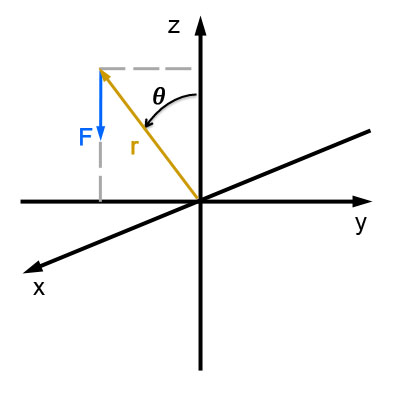
\includegraphics[width=0.4\textwidth]{ImgTorqueSol.jpg}
%  \end{center}
%\end{figure}
%\BEN
%\item Using the above coordinate system, we are given that $||\MB{r}|| = 0.14$ and $\MB{F} = -100\MB{k}$. Also, 
%\begin{align*}
%  \MB{r} &=- \sin(30^{\circ})||\MB{r}||\MB{j} + \cos(30^{\circ} )||\MB{r}||\MB{k}\\
%  &= -0.07\MB{j} + 0.07\sqrt{3}\MB{k}\\
%  &= 0.07\big(-\MB{j} + \sqrt{3}\MB{k}\big)
%\end{align*}
%To compute the torque when $\theta = 30^{\circ}$, we use the cross product:
%\begin{align*}
%0.07
%\begin{vmatrix}
%   \MB{i} & \MB{j} &  \MB{k} \\
%   0 & -1 &  \sqrt{3} \\
%   0 & 0 & -100  \\
%  \end{vmatrix}=7\MB{i}
%\end{align*} 
%Thus, the magnitude of the torque $\boldsymbol\tau$ is 7 N$\cdot$m. A similar calculation for $\theta = 90^{\circ}$ yields a magnitude of 14 N$\cdot$m
%% ~  ~  ~  ~  ~  ~  ~  ~  ~  ~  ~  ~  ~  ~  ~  ~  ~  ~  ~  ~  ~  ~  ~  ~  ~  ~  ~  
%\item Using a similar calculation from above, 
%\begin{align*}
%  \MB{r} &=- \sin\theta||\MB{r}||\MB{j} + \cos\theta||\MB{r}||\MB{k}\\
%  &= -0.14\sin\theta\MB{j} + 0.14\cos\theta\MB{k}
%\end{align*}
%To compute the torque when $\theta = 30^{\circ}$, we use the cross product:
%\begin{align*}
%0.14
%\begin{vmatrix}
%   \MB{i} & \MB{j} &  \MB{k} \\
%   0 & -\sin\theta &  \cos\theta \\
%   0 & 0 & -100  \\
%  \end{vmatrix}=14\sin\theta\MB{i}
%\end{align*} 
%Thus, the magnitude of the torque $\boldsymbol\tau$ is $|| 14\sin\theta\MB{i} || \text{N}\cdot\text{m} = 14 |\sin\theta|$N$\cdot$m.
%% ~  ~  ~  ~  ~  ~  ~  ~  ~  ~  ~  ~  ~  ~  ~  ~  ~  ~  ~  ~  ~  ~  ~  ~  ~  ~  ~  
%\item The magnitude is minimized when $\theta = 0$ or $180^{\circ}$. This corresponds to angles when $\MB{F}$ and $\MB{r}$ are parallel (or anti-parallel). The cross product of two vectors that are parallel (or anti-parallel) is zero.  
%\EEN
%
%%%%%%%%%%%%%%%%%%%%%%%%%%%%%%%%%%%%%%%
%%%%%%%%%%%%%%%%%%%%%%%%%%%%%%%%%%%%%%%
%%%%%%%%%%%%%%%%%%%%%%%%%%%%%%%%%%%%%%%
%
\EEN

